\section{Structure of the document}

\begin{figure}
	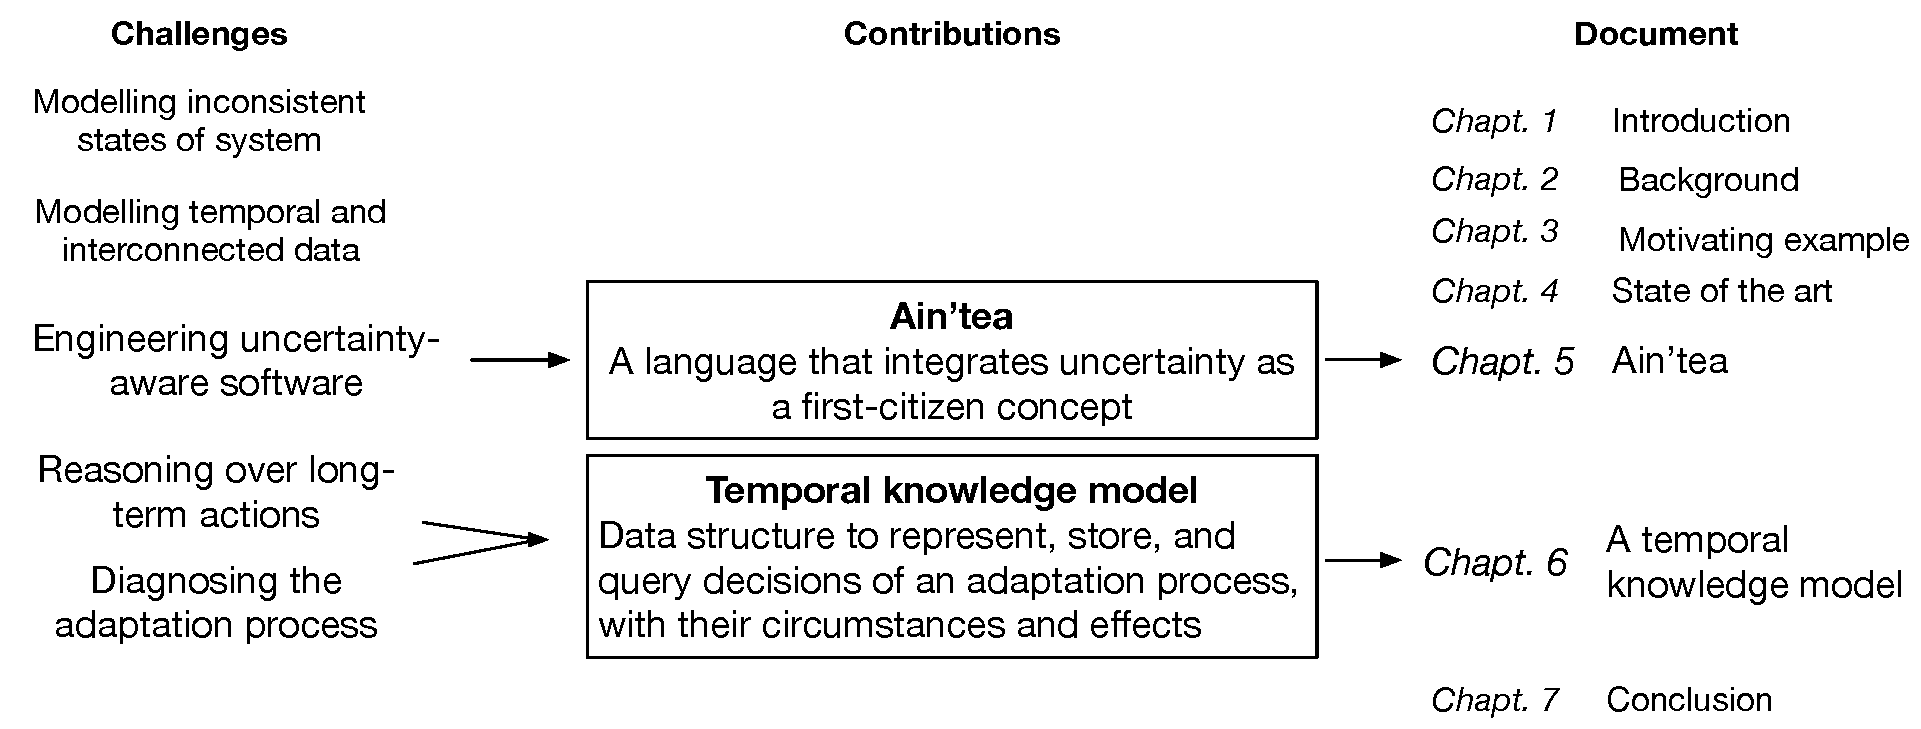
\includegraphics[width=\linewidth]{img/chapt-intro/struct/struct}
	\caption{Structure of the document}
	\label{fig:intro:structDoc}
\end{figure}

We split the remaining part of this document into seven chapters, as shown in~\Cref{fig:intro:structDoc}.
First, \Cref{chapt:background} describes the necessary background of the thesis.
Then, \Cref{chapt:example} describes a motivating example, based on a \gls{sg} system.
We present concepts related to \gls{mde} and \glspl{adptSyst}.
Based on this background, we show the gap of the current state of the art in \Cref{chapt:sota}.
\Cref{chapt:vision} explains our vision.
\Cref{chapt:aintea} and \Cref{chapt:tkm} describe our two contributions.
The former details our language, \langName, that integrates uncertainty as a first-class citizen.
The latter explains our temporal \gls{metamodel} that can represent past and ongoing \glspl{action} with their circumstances and effects.
Finally, we conclude in \Cref{chapt:conclusion}, and we present future work.